\documentclass[conference]{IEEEtran}
\IEEEoverridecommandlockouts
\usepackage{cite}
\usepackage{amsmath,amssymb,amsfonts}
\usepackage{algorithmic}
\usepackage{mathpazo}
\usepackage[spanish]{babel}
\usepackage[utf8]{inputenc}
\usepackage[T1]{fontenc}
\usepackage{graphicx}
\usepackage{textcomp}
\usepackage{xcolor}
%\usepackage{minted}
%\usemintedstyle{emacs}
\usepackage{url}
\usepackage{ctable}
\usepackage{float}
\usepackage{amsmath,amssymb,amsfonts}
\usepackage{makecell}
\usepackage{hyperref}
\usepackage{comment}
\hypersetup{
	colorlinks=true,
	linkcolor=blue,
	filecolor=magenta,      
	urlcolor=cyan,
}
\newcommand{\DNoise}{n_d}

\newcommand{\Est}[1]{\hat{#1}}
\newcommand{\Test}[1]{\expandafter\hat#1}

\def\BibTeX{{\rm B\kern-.05em{\sc i\kern-.025em b}\kern-.08em
    T\kern-.1667em\lower.7ex\hbox{E}\kern-.125emX}}
    
\begin{document}
\title{\bf{Consultas SparQl a estructuras RDF}}

\begin{comment}
\author{\IEEEauthorblockN{Asmat Franco, Bryan}
\IEEEauthorblockA{\textit{Universidad Nacional de Ingeniería} \\
Lima, Perú \\
\texttt{basmatf@uni.pe}}
\and
\IEEEauthorblockN{Blas Salas, Israel}
\IEEEauthorblockA{\textit{Universidad Nacional de Ingeniería} \\
Lima, Perú \\
\texttt{iblass@uni.pe}}
\and
\IEEEauthorblockN{Chavez Bruno, Victor}
\IEEEauthorblockA{\textit{Universidad Nacional de Ingeniería} \\
Lima, Perú \\
\texttt{vchavezb@uni.pe}}
\and
\IEEEauthorblockN{Guadalupe Quispe, William}
\IEEEauthorblockA{\textit{Universidad Nacional de Ingenieri\'a} \\
Lima, Perú \\
\texttt{wguadalupeq@uni.pe}}
}
\end{comment}
\author{%x  x
\textsc{Bryan Asmat}\textsc{, Danilo Blas}\textsc{, Victor Chavez}\textsc{, William Guadalupe}\\
%\thanks{A thank you or further information} \\[1ex] % Your name
\normalsize Universidad Nacional de Ingenieria \\ % Your institution
\normalsize Lima,Perú \\ % Your institution
\normalsize \href{mailto:basmatf@uni.pe}{basmatf@uni.pe},  \href{mailto:iblass@uni.pe}{iblass@uni.pe} \href{mailto:vchavezb@uni.pe}{,  vchavezb@uni.pe} \href{mailto:wguadalupeq@uni.pe}{,  wguadalupeq@uni.pe} % Your email address
%\and % Uncomment if 2 authors are required, duplicate these 4 lines if more
%\textsc{Jane Smith}\thanks{Corresponding author} \\[1ex] % Second author's name
%\normalsize University of Utah \\ % Second author's institution
%\normalsize \href{mailto:jane@smith.com}{jane@smith.com} % Second author's email address
}





\maketitle

\begin{abstract}
La información en la web se puede representar bajo un formato de datos llamado RDF

En el presente trabajo se implementaron consultas de tipos SPARQL que permiten hacer la busqueda en distintas fuentes de datos.

\vspace{0.2cm}


\'Indice de T\'erminos— RNN, modelos seq2seq, mecanismos de atenci\'on, transformers.
    
\end{abstract}

\section{Introducci\'on}
Una tendencia dada en el ICRL \footnote{International Conference on Learning Representations } y en el NAACL- HLT \footnote{Annual Conference of the North American Chapter of the Association for Computational Linguistics: Human Language Technologies.} celebrados en el 2019,  muestra que las RNN presentan un declive en el n\'umero de publicaciones realizadas. Dicha tendencia era de esperarse, aunque las RNN son intuitivas para los datos secuenciales tienen como principal incoveniente la parelización en su procesamiento, por lo tanto, no pueden aprovechar el factor m\'as importante que ha impulsado el progreso en la investigaci\'on desde $2012$: la potencia de c\'alculo. Los RNN nunca han sido populares en visi\'on computacional y aprendizaje por refuerzo y para NLP, est\'an siendo reemplazados por arquitecturas basadas en la atenci\'on.

\vspace{0.2cm}

Los Transformers, presentados en 2017, introdujeron un nuevo enfoque: m\'odulos de atenci\'on. Este modelo ha conllevado a una enorme cantidad de variantes que mejoran el desempe\~no de tareas del NLP, como el Transformer Universal, BERT (google) o el Transformer-XL; la mayor\'ia de modelos de vanguardia que requieren gran cantidad de datos de entrenamiento y d\'ias de entrenamiento en hardware haci\'endolo costoso. Sin embargo, con el lanzamiento de librer\'ias especializadas en NLP y arquitecturas Transformer, ahora pueden ser utilizados en datos reducidos.

\vspace{0.2cm}

De esta manera, el presente trabajo busca explorar la aplicación de estos modelos sobre el conjunto de datos reducido AG News y Multi30k. En primer lugar se realizar\'a la definici\'on del modelo Transformer. A continuaci\'on, se describir\'a el estado del arte de modelos basados en el Transformer, para diferentes tareas del NLP. Posteriomente, se explica la metodolog\'ia a utilizar en los experimentos con diferentes arquitecturas. Las secciones siguientes tratar\'an los resultados experimentales, las conclusiones y discusiones, y los trabajos futuros que se pueden realizar con esta nueva familia de t\'ecnicas del NLP.

\vspace{0.2cm}

\section{Estructura RDF}
RDF representa la información en una declaración triple -también llamada tripleta- que sigue la estructura sujeto-predicado-objeto
 \textcolor{orange}{Attention Is All You Need} \cite{b1}, se basa en la auto-atenci\'on sin el uso de RNN. Como resultado, es altamente paralelo y requiere menos tiempo para entrenamiento, al tiempo que establece resultados de vanguardia en modelamiento de lenguaje y la traducci\'on autom\'atica.

\vspace{0.2cm}

El Transformer se basa en una estructura encoder-decoder. La diferencia entre este y cualquier otro modelo es que el Transformer se basa completamente en mecanismos de atenci\'on. 

\begin{figure}[h]
%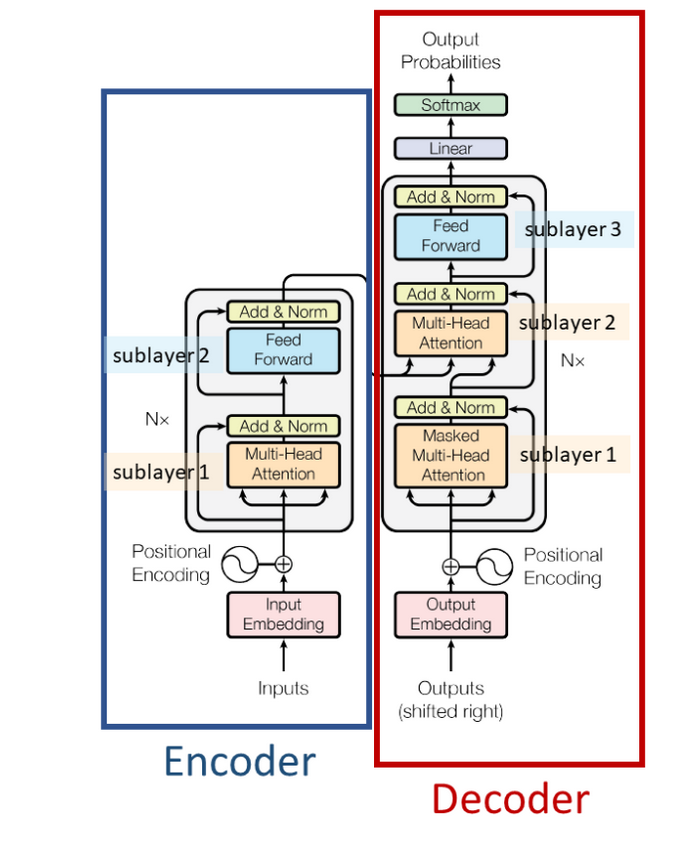
\includegraphics[scale=0.3]{imagenes/Encoder-decoder.png} 
\caption{Encoder-Decoder del Transformer. Fuente The Transformer:
Attention Is All You Need. \cite{b1}}
\end{figure}

\vspace{0.2cm}


El encoder est\'a formado por una pila de $N = 6$ capas, cada una de las cuales est\'a compuesta por dos subcapas: un mecanismo de atenci\'on de m\'ultiples cabeceras y una red de alimentaci\'on directa completamente conectada m\'as conexiones residuales \cite{b2} en ambas etapas, seguidas de un procedimiento de normalizaci\'on de capas \cite{b3}. El decoder se define de manera similar, solo que cada capa est\'a compuesta de 3 subcapas: atenci\'on de m\'ultiples cabeceras, capas completamente conectadas y atenci\'on de m\'ultiples cabeceras enmascarada.

\vspace{0.2cm}

Este modelo fue entrenado durante $300000$ pasos, aproximadamente $3.5$ d\'ias, utilizando \texttt{8 GPU NVIDIA P100}. De esta manera, el modelo Transformer alcanz\'o un puntaje BLUE \cite{b4} de $26.4$ cuando se aplic\'o sobre el conjunto de datos \texttt{newstest2013} como un conjunto de prueba, que estableci\'o un nuevo resultado de vanguardia.
\vspace{0.2cm}

El Transformer es una mejora con respecto a los modelos seq2seq basados en RNN, pero tiene algunas limitaciones.

\begin{itemize}
\item La atenci\'on solo puede ocuparse de cadenas de texto de longitud fija, lo cual implica que el texto debe dividirse en un cierto n\'umero de segmentos antes de ser alimentado al sistema como entrada. 

\item Esta segmentaci\'on del texto provoca la fragmentaci\'on del contexto \footnote{Context fragmentation}. Por ejemplo, si una oraci\'on se divide en dos, se pierde una cantidad significativa de contexto. En otras palabras, el texto se divide sin considerar la oraci\'on o cualquier otro l\'imite sem\'antico.
\end{itemize}
\section{COnsultas SPARQL}
Con la aparici\'on del Transformer, han surgido diversas variantes y mejoras del modelo para  mejorar las limitaciones  y el desempe\~no en diversas tareas del NLP. En esta secci\'on describiremos algunas relacionadas a este trabajo.

\subsection{Transformer Universal}

El Transformer Universal, propuesto en el art\'iculo del mismo nombre \textcolor{orange}{Universal Transformers} \cite{b5}, es una variante del modelo Transformer que tiene como objetivo lograr un buen rendimiento tanto en traducci\'on de lenguaje como en tareas algor\'itmicas con un solo modelo. Los autores del Transformer Universal se\~nalan que es un modelo completo de Turing. 

\vspace{0.2cm}

De acuerdo al art\'iculo, las principales diferencias entre el Transformer y el Transformer Universal consistn en que el Transformer Universal aplica el encoder para un n\'umero variable de pasos para cada token de entrada/salida (T pasos), mientras que el Transformador aplica exactamente $6$ capas de encoder/decoder, respectivamente. As\'i mismo, el Transformer Universal utiliza una representaci\'on de entrada ligeramente diferente: incluye un embedding de paso de tiempo adem\'as de la codificaci\'on posicional.

\vspace{0.2cm}

Los n\'umeros variables de pasos presentes en el Transformer Universal se logran mediante el uso de \textcolor{green}{Adaptive Computation Time}, un mecanismo propuesto por Alex Graves \cite{b6} que permite la aplicaci\'on del encoder y decoder un n\'umero variable de veces.
	
\vspace{0.2cm}

\subsection{Transformer-XL}

El transformer-XL es uno de los primeros modelos exitosos en abordar el problema de poseer una longitud fija en la secuencia de entrada. En el art\'iculo \textcolor{orange}{Transformer-XL: Attentive Language Models Beyond a Fixed-Length Context} \cite{b7} se propone este m\'etodo novedoso para el modelado de lenguaje, que permite que una arquitectura transformer aprenda dependencia a largo plazo, a trav\'es de un mecanismo de recurrencia, m\'as all\'a de una longitud fija sin alterar la coherencia temporal.

\vspace{0.2cm}

Se introduce un mecanismo recurrente a nivel de segmento que permite que el modelo reutilice estados ocultos anteriores en el momento del entrenamiento, abordando tanto los problemas del contexto de longitud fija como la fragmentaci\'on del contexto. En otras palabras, la informaci\'on hist\'orica se puede reutilizar y se puede extender tanto como lo permita la memoria de la GPU.
	
\vspace{0.2cm}

Para reutilizar adecuadamente los estados ocultos, los autores proponen un mecanismo llamado codificaciones posicionales relativas  que ayuda a evitar la confusi\'on temporal. Los modelos actuales no pueden distinguir la diferencia posicional entre entradas en diferentes segmentos en diferentes capas. La codificaci\'on de posici\'on relativa soluciona este problema al codificar el sesgo de informaci\'on posicional en los estados ocultos, que difiere de otros enfoques que realizan esto como el nivel de entrada.

\begin{figure}[h]
%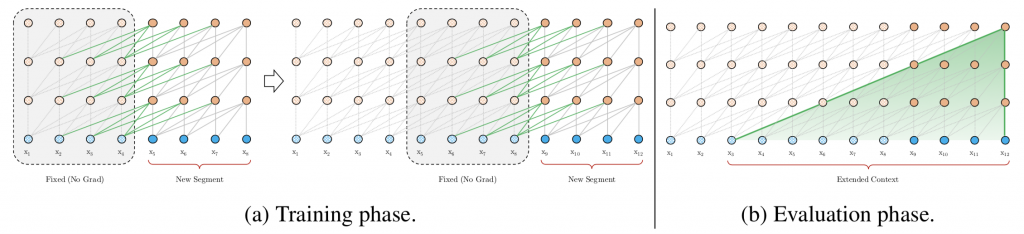
\includegraphics[scale=0.25]{imagenes/TransformerXL1.png} 
\caption{Transformer XL: Entrenamiento y Evaluación. Fuente: Transformer XL \cite{b7}}
\end{figure}


\vspace{0.2cm}


El transformer-XL reduce el puntaje de perplejidad SoTA anterior en varios conjuntos de datos como text8, enwiki8, One Billion Word y WikiText-103. Los autores afirman que el m\'etodo es m\'as flexible, m\'as r\'apido durante la evaluaci\'on (aceleraci\'on de $1874$ veces), se generaliza bien en conjuntos de datos peque\~nos y es eficaz para modelar secuencias cortas y largas.

\vspace{0.2cm}

As\'i mismo, los autores proponen una nueva m\'etrica llamada Relative Effective Context Length que proporciona una manera justa de comparar modelos que se prueban con mayores longitudes de contexto.

\subsection{XLNet}

XLNet es un modelo presentado en el art\'iculo \textcolor{green}{XLNet: Generalized Autoregressive Pretraining for Language Understanding} \cite{b8} que es un lenguaje autoregresivo que genera la probabilidad conjunta de una secuencia de tokens basada en la arquitectura del Transformer con recurrencia. Este modelo introduce una variante de modelado de lenguaje llamada modelado de lenguaje de permutaci\'on. Los modelos de lenguaje de permutaci\'on est\'an entrenados para predecir un token dado el contexto anterior como el modelo de lenguaje tradicional, pero en lugar de predecir los tokens en orden secuencial, predice los tokens en un orden aleatorio.

\vspace{0.2cm}

Adem\'as de usar el modelado de lenguaje de permutaci\'on, XLNet mejora BERT  al usar el Transformer XL como su arquitectura base. XLNet utiliza las dos ideas clave de Transformer XL: embeddings posicionales relativas y el mecanismo de recurrencia. Los estados ocultos del segmento anterior se almacenan en cach\'e y se congelan mientras se realiza el modelado del lenguaje de permutaci\'on para el segmento actual. Como todas las palabras del segmento anterior se usan como entrada, no es necesario conocer el orden de permutaci\'on del segmento anterior.
	
\subsection{BERT}

Este modelo \cite{b9},publicado el 2018, esta conformado por una pila de bloques Transformers, la cual esta pre-entrenada en un corpus de dominio general con 800 millones de palabras. 
Este modelo obtiene un mejor rendimiento que modelos anteriores a su publicación debido a su naturaleza bidireccional donde la atención se centra en toda la secuencia. 

\subsection{RoBERTa}

Es un modelo introducido en Facebook. El enfoque BERT robustamente optimizado RoBERTa \cite{b10}, es un reentrenamiento de BERT con una metodolog\'ia de entrenamiento mejorada, un $1000\%$ más de datos y potencia de cálculo. Para mejorar el procedimiento de entrenamiento, RoBERTa elimina tareas como Next Sentence Prediction (NSP) del entrenamiento previo de BERT e introduce el enmascaramiento dinámico para que el token enmascarado cambie durante las \'epocas de entrenamiento. 

\vspace{0.2cm}

RoBERTa supera a BERT y XLNet en los resultados de referencia de \href{https://gluebenchmark.com/}{GLUE}.

\subsection{DistilBERT}

Este modelo aprende una versión destilada (aproximada) de BERT, que retiene el $95\%$ de rendimiento pero utiliza solo la mitad del n\'umero de par\'ametros. Espec'ificamente, no tiene embeddings de tipo token, pooler y retiene solo la mitad de las capas del BERT de Google.

DistilBERT \cite{b11}, utiliza una técnica llamada destilation, que se aproxima a BERT de Google. La idea es que una vez que se ha entrenado una gran red neuronal, sus distribuciones de salidas completas se pueden aproximar usando una red más pequeña. Una de las funciones clave de optimización utilizadas para la aproximación posterior en las estadísticas bayesianas es la divergencia de Kulback-Leiber.

\section{Conclusiones}

\begin{itemize}
\item Se ha realizado clasificaci\'on multiclase utilizando la librer\'ia simpletransformers y modelos pre-entrenados, basados en BERT, obteniendo buenos resultados en m\'etricas de clasificaci\'on, especialmente del modelo distilBERT, que tiene un menor n\'umero de param\'etros que BERT y que utiliza el aprendizaje \texttt{teacher-students}, donde se entrena a una red de \texttt{students} para imitar la distribuci\'on de salida completa de la red del \texttt{teacher} (su conocimiento) y retiene el rendimiento de BERT.
\item En la tarea de traducci\'on, se realizaron comparaciones entre distintos modelos seq2seq y los modelos transformers, donde estos \'ultimos obtuvieron mejores resultados. Sin embargo el modelo Transformer XL modificado no logr\'o superar al Transformer original.
\end{itemize}

%\section{Referencias}
\begin{thebibliography}{00}

\bibitem{b1} Vaswani, Ashish, Noam Shazeer, Niki Parmar, Jakob Uszkoreit, Llion Jones, Aidan N. Gomez, Łukasz Kaiser, and Illia Polosukhin. Attention is all you need. In 
\bibitem{b2}Sergey Ioffe, Christian Szegedy. Batch Normalization: Accelerating Deep Network Training by Reducing Internal Covariate Shift (2015). Disponible en \href{https://arxiv.org/abs/1502.03167}{https://arxiv.org/abs/1502.03167}.
\bibitem{b3} Jimmy Lei Ba, Jamie Ryan Kiros, Geoffrey E.Hinton. Layer Normalization (2016). Disponible en \href{https://arxiv.org/abs/1607.06450}{https://arxiv.org/abs/1607.06450}.
\bibitem{b4}Kishore Papineni , Salim Roukos , Todd Ward , Wei-jing Zhu (2002). BLEU: a Method for Automatic Evaluation of Machine Translation,  pp. 311-318. Proceedings of the 40th Annual Meeting of the Association for Computational Linguistics (ACL). 
\bibitem{b5}Mostafa Dehghani, Stephan Gouws, Oriol Vinyals, Jakob Uszkoreit, Łukasz Kaiser. Universal Transformers (2018). ICLR 2019. Disponible en \href{https://arxiv.org/abs/1807.03819}{https://arxiv.org/abs/1807.03819}
\bibitem{b6}Alex Graves. Adaptive Computation Time for Recurrent Neural Networks (2017). Disponible en \href{https://arxiv.org/abs/1603.08983}{https://arxiv.org/abs/1603.08983}.
\bibitem{b7}Zihang Dai, Zhilin Yang, Yiming Yang, Jaime Carbonell, Quoc V. Le, Ruslan Salakhutdinov. Transformer-XL: Attentive Language Models Beyond a Fixed-Length Context (2019). Disponible en \href{https://arxiv.org/abs/1901.02860}{https://arxiv.org/abs/1901.02860}. 
\bibitem{b8}Zhilin Yang, Zihang Dai, Yiming Yang, Jaime Carbonell, Ruslan Salakhutdinov, Quoc V. Le. XLNet: Generalized Autoregressive Pretraining for Language Understanding (2019). Disponible en \href{https://arxiv.org/abs/1906.08237}{https://arxiv.org/abs/1906.08237}.
\bibitem{b9}Jacob Devlin, Ming-Wei Chang, Kenton Lee, Kristina Toutanova. BERT: Pre-training of Deep Bidirectional Transformers for Language Understanding (2018). Disponible en \href{https://arxiv.org/abs/1810.04805}{https://arxiv.org/abs/1810.04805}.
\bibitem{b10}Yinhan Liu, Myle Ott, Naman Goyal, Jingfei Du, Mandar Joshi, Danqi Chen, Omer Levy, Mike Lewis, Luke Zettlemoyer, Veselin Stoyanov- RoBERTa: A Robustly Optimized BERT Pretraining Approach (2019). Disponible en \href{https://arxiv.org/abs/1907.11692}{https://arxiv.org/abs/1907.11692}.
\bibitem{b11}Victor Sanh, Lysandre Debut, Julien Chaumond, Thomas Wolf. DistilBERT, a distilled version of BERT: smaller, faster, cheaper and lighter (2019). Disponible en \href{https://arxiv.org/abs/1910.01108}{https://arxiv.org/abs/1910.01108}.
\bibitem{b12}Pytorch-Transform:Implementaci\'on de transformer para NLP. \href{https://pytorch.org/hub/huggingface\_pytorch-transformers/}{https://pytorch.org/hub/huggingface\_pytorch-transformers/}.
\bibitem{b13}Thomas Wolf, Lysandre Debut, Victor Sanh, Julien Chaumond,
Clement Delangue, Anthony Moi, Pierric Cistac, Tim Rault,
R\'emi Louf, Morgan Funtowicz, Jamie Brew. Transformers: State-of-the-art Natural
Language Processing (2019), HuggingFace Inc. Disponible en \href{https://arxiv.org/abs/1910.03771}{https://arxiv.org/abs/1910.03771}.
\bibitem{b14}SimpleTransformers \href{https://pypi.org/project/simpletransformers/}{https://pypi.org/project/simpletransformers/}.
\bibitem{b15} Xiang Zhang, Junbo Zhao, Yann LeCun. 
Character-level Convolutional Networks for Text Classification(2015). Disponible en \href{https://arxiv.org/abs/1509.01626}{https://arxiv.org/abs/1509.01626}. 
\bibitem{b16} Desmond Elliott, Stella Frank, Khalil Sima'an, Lucia Specia. 
Multi30K: Multilingual English-German Image Descriptions(2016). Disponible en \href{https://arxiv.org/abs/1605.00459}{https://arxiv.org/abs/1605.00459}. 
\bibitem{b17}TransformerXL from Scratch \href{https://github.com/keitakurita/Practical_NLP_in_PyTorch/blob/master/deep_dives/transformer_xl_from_scratch.ipynb}{notebook}.
\end{thebibliography}

\end{document}
